	\chapter{Installation Notes}
\codetext{!\{sys.executable\} -m pip install pandas-profiling}

Use this to import from another directory.
	\begin{code}[\codenumbering]{}
		\codeitemnonumber import sys
		\codeitemnonumber sys.path.insert(1, "..\textbackslash{}lendres\textbackslash{}")
	\end{code}


Code folding:
https://jupyter-contrib-nbextensions.readthedocs.io/en/latest/install.html

\textcode{conda install -c conda-forge jupyter\_contrib\_nbextensions}
	\begin{figure}[tbp]
		\centering
		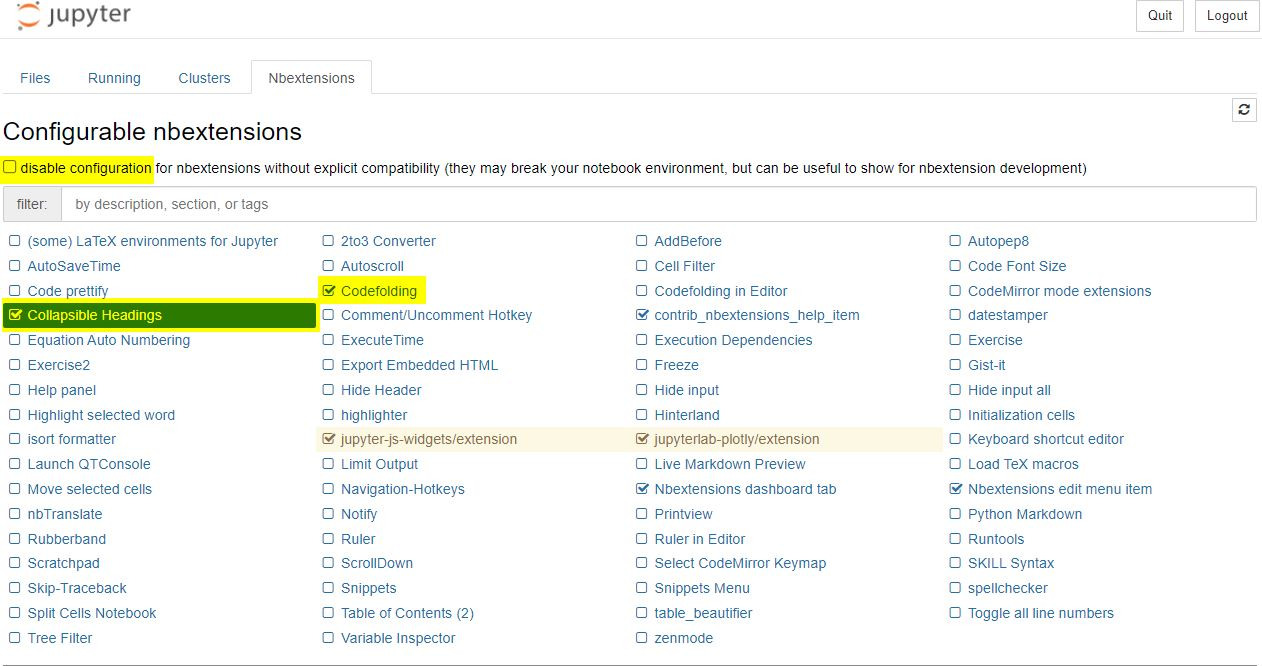
\includegraphics[width=\textwidth]{jupyterenablefolding}
		\caption{Enable nbextensions for Jupyter notebooks.}
		\label{fig:normaldistrution}
	\end{figure}


	\section{Imbalanced}
	\begin{code}[\codenumbering]{}
		\codeitemnonumber \# Jupyter notebook
		\codeitemnonumber !pip install imblearn --user
		\codeitemnonumber !pip install imbalanced-learn --user
		\codeitemnonumber
		\codeitemnonumber \# Anaconda prompt
		\codeitemnonumber \#!pip install -U imbalanced-learn

		\codeitemnonumber \#conda install -c conda-forge imbalanced-learn

		\codeitemnonumber \# Restart the kernel after successful installation of the library
	\end{code}

	\section{Anaconda and Python}
	\begin{code}[\codenumbering]{}
		\codeitemnonumber conda update -n base conda
		\codeitemnonumber conda update --all
		\codeitemnonumber jupyter contrib nbextension install --user
	\end{code}

\textcode{conda install -c conda-forge sklearn-pandas}

	\section{Jupyter Notebooks}
	\subsection{Version}
\textcode{jupyter --version}

	\subsection{Original Start Up Short Cut}
Original short cut target value:
	\begin{code}[\codenumbering]{}
		\codeitemnonumber F:\textbackslash{}anaconda3\textbackslash{}python.exe F:\textbackslash{}anaconda3\textbackslash{}cwp.py F:\textbackslash{}anaconda3 F:\textbackslash{}anaconda3\textbackslash{}python.exe F:\textbackslash{}anaconda3\textbackslash{}Scripts\textbackslash{}jupyter-notebook-script.py "\%USERPROFILE\%/"
	\end{code}

\noindent Original start in value:
	\begin{code}[\codenumbering]{}
		\codeitemnonumber \%HOMEPATH\%
	\end{code}


	\subsection{Changing Jupyter Start Up Location}
This section shows how to change the default Jupyter start up folder.  This information was take from:\\
{\small \url{https://stackoverflow.com/questions/35254852/how-to-change-the-jupyter-start-up-folder}}

	\subsubsection{Jupyter Notebook and JupyterLab $<$ 3.0 Versions}
	\begin{numberedlist}
		\item Use \textcode{Run as Administrator} on the Anaconda Powershell Prompt.
		\item At the command prompt run:\\ \textcode{jupyter notebook --generate-config}. \label{nl:jupyterstartupfoldergenerateconfiguration}
		\item Open the written by the command in the previous step.  The file location is specified as output from the command.  Typically, it is This writes a file to:\\ \textcode{C:\textbackslash{}Users\textbackslash{}username\textbackslash{}.jupyter\textbackslash{}jupyter\_notebook\_config.py} \label{nl:jupyterstartupfolderconfigurationfile}
		\item Search for the following line in the file:\\ \textcode{\#c.NotebookApp.notebook\_dir = \textquoteright{}\textquoteright{}} \label{nl:jupyterstartupfoldersearchforline}
		\item Uncomment the line.
		\item Edit the path\footnote{\warning{Be sure to use forward slashes instead of back slashes in the path.}} to the desired location, for example:\\ \textcode{c.NotebookApp.notebook\_dir = "C:/Projects/Python/"}  \label{nl:jupyterstartupfoldereditpath}
		\item From the start menu, right click on the Jupyter Notebook tile and select:\\ \textcode{More->Open File Location}
		\item From the file explorer window that opened, right click on the Jupyter Notebook short cut and select \textcode{Properties}.
		\item In the \textcode{Target} text box, go to the end of the line and delete:\\ \textcode{"\%USERPROFILE\%/"}
		\item Click the \textcode{Apply} button.  If prompted that administrator rights are required, confirm that you want to continue.
		\item Click the \textcode{Ok} button.
	\end{numberedlist}

	\subsubsection{JupyterLab $\geq$ 3, Jupyter Notebook Classic, and RetroLab}
	\begin{bulletedlist}
		\item In step~\ref{nl:jupyterstartupfoldergenerateconfiguration} above, replace:\\ \textcode{jupyter notebook --generate-config}\\ with\\ \textcode{jupyter server --generate-config}.
		\item In step~\ref{nl:jupyterstartupfolderconfigurationfile} above, the file written is typically:\\ \textcode{jupyter\_server\_config.py}

		\item In steps~\ref{nl:jupyterstartupfoldersearchforline} and~\ref{nl:jupyterstartupfoldereditpath} above, the configuration line:\\ \textcode{c.NotebookApp.notebook\_dir}\\ is instead:\\ \textcode{c.ServerApp.root\_dir}
	\end{bulletedlist}


	\section{Imblearn library}
To install imblearn you can use:
	\begin{code}[\codenumbering]{}
		\codeitemnonumber !pip install imbalanced-learn==0.8.0 \# In Jupyter notebook
		\codeitemnonumber pip install imbalanced-learn==0.8.0 \# In anaconda prompt
	\end{code}


	\section{SMOTE}
I am getting this error while trying to import SMOTE, how do I fix it?

\noindent\textcode{ImportError: cannot import name `delayed' from `sklearn.utils.fixes' (C:\textbackslash{}Users\textbackslash{}anaconda3\textbackslash{}lib\textbackslash{}site-packages\textbackslash{}sklearn\textbackslash{}utils\textbackslash{}fixes.py)}

Use the following:
	\begin{code}[\codenumbering]{}
		\codeitemnonumber !pip install imbalanced-learn==0.8.0
		\codeitemnonumber !pip install delayed
	\end{code}


	\section{Yellowbrick}
\textcode{conda install -c districtdatalabs yellowbrick}
\textcode{python -m pip install yellowbrick}


	\section{Google Colab GPUs}
\textcode{Edit->Notebook Settings->Hardware Acceleration}

\textcode{!pip list}

from google.colab import drive
drive.mount("/content/drive") 